\documentclass[review]{elsarticle}

\usepackage{lineno,hyperref}
\usepackage{pdflscape}
\modulolinenumbers[5]

\journal{Geochemica and Cosmochemica Acta}

%%%%%%%%%%%%%%%%%%%%%%%
%% Elsevier bibliography styles
%%%%%%%%%%%%%%%%%%%%%%%
%% To change the style, put a % in front of the second line of the current style and
%% remove the % from the second line of the style you would like to use.
%%%%%%%%%%%%%%%%%%%%%%%

%% Numbered
%\bibliographystyle{model1-num-names}

%% Numbered without titles
%\bibliographystyle{model1a-num-names}

%% Harvard
\bibliographystyle{model2-names.bst}\biboptions{authoryear}

%% Vancouver numbered
%\usepackage{numcompress}\bibliographystyle{model3-num-names}

%% Vancouver name/year
%\usepackage{numcompress}\bibliographystyle{model4-names}\biboptions{authoryear}

%% APA style
%\bibliographystyle{model5-names}\biboptions{authoryear}

%% AMA style
%\usepackage{numcompress}\bibliographystyle{model6-num-names}

%% `Elsevier LaTeX' style
%\bibliographystyle{elsarticle-num}
%%%%%%%%%%%%%%%%%%%%%%%

\begin{document}

\begin{frontmatter}

\title{The compositions of high-pressure water-rich melts in the system MgO-SiO$_2$-H$_2$O}
%\tnotetext[mytitlenote]{Fully documented templates are available in the elsarticle package on \href{http://www.ctan.org/tex-archive/macros/latex/contrib/elsarticle}{CTAN}.}

%% Group authors per affiliation:
\author{R. Myhill, D. J. Frost}
\address{Bayerisches Geoinstitut, Universit\"{a}t Bayreuth, Universit\"{a}tsstrasse 30, 95447 Bayreuth, Germany}
\cortext[mycorrespondingauthor]{Corresponding author: R. Myhill}
\ead{myhill.bob@gmail.com}

\author{D. Novella}
\address{Laboratoire Magmas et Volcans, Universit\'{e} Blaise Pascal, 5 Rue Kessler, 63038 Clermond-Ferrand, France}

%% or include affiliations in footnotes:
%\author[mymainaddress,mysecondaryaddress]{Elsevier Inc}
%\ead[url]{www.elsevier.com}

%\author[mysecondaryaddress]{Global Customer Service\corref{mycorrespondingauthor}}

%\address[mymainaddress]{1600 John F Kennedy Boulevard, Philadelphia}
%\address[mysecondaryaddress]{360 Park Avenue South, New York}

\begin{abstract}
High pressure multianvil experiments were conducted at 13 GPa between 1200 and 1900 $^{\circ}$C to investigate the liquidus in the system MgO-SiO$_2$-H$_2$O. Water-rich starting compositions were obtained by using platinic acid (H$_2$Pt(OH)$_6$) as a novel water source. The topology of the liquidus is tightly constrained at much higher water contents than previously possible. In the subsystem MgO-H$_2$O, the invariant point between brucite, periclase and liquid occurs at ca. 1210 $^{\circ}$C and 67 mol\% H$_2$O. Forsterite and clinoenstatite both melt congruently in the temperature range investigated, although the fo-cen and cen-stv cotectics migrate close to the fo-H$_2$O and cen-H$_2$O binaries at high water contents. The chondrodite liquidus field approaches the fo-H$_2$O binary at ca. 1200 $^{\circ}$C. Preliminary experiments on the SiO$_2$-H$_2$O binary reveal a pronounced melting point depression up to about 20 mol\% H$_2$O, then shallowing up to 50 mol\%, similar to behaviour previously observed at 2 GPa.
\end{abstract}

\begin{keyword}
high pressure \sep mantle \sep hydrous melting \sep water \sep liquidus
\end{keyword}

\end{frontmatter}

\linenumbers

\section{Introduction}
The subduction of hydrous materials has a strong influence on the formation of melts within the deep Earth. The dehydration of hydrous crustal minerals is thought to drive the melting of the mantle wedge that feeds arc volcanoes. Dehydration of the underlying lithospheric mantle may also enable embrittlement of the slab, allowing it to deform at significantly higher strain rates than would be possible if it were dry. 

There has been some controversy over whether slabs transport water beyond about 300 km depth. Certainly most of the ca. 7 km thick mafic crust is probably too warm to sustain hydrous minerals. However, hydrated ultramafics can potentially carry water into the lower mantle. Supporting evidence for an ultradeep part of the water cycle exists in the form of hydrous ringwoodite in diamond, which apparently formed under cold conditions. 

The compositions of melts formed by the breakdown of hydrous phases is important for a full understanding of the deep water system. The thermodynamics of melting in water-rich systems cannot be determined without good estimates of melt compositions. Furthermore, the thermal stability of hydrous phases cannot be predicted from their properties without also having an activity-composition model for the melt phase. More generally, the density of hydrous melts will be highly composition dependent, impacting on their ability to rise through the mantle. Finally, reactions between migrating melts and the surrounding solid will be controlled by the \emph{P-T-X} dependence on melt composition.

Although the phase relations in hydrous systems in the upper mantle are now remarkably well-constrained, constraining melt compositions has remained a major challenge in high-pressure experimental petrology. The primary problem is that hydrous melts are unquenchable, which means that their compositions must be estimated indirectly. Compositions of partial hydrous melts have been estimated using mass balance, diamond traps \citep{MSUP2007}, and the Mg:Si ratio has been estimated by defocusing the beam of an electron probe microanalyser (EPMA) \citep[e.g.][]{YII2004}. Unfortunately, all three of these techniques are accompanied by significant uncertainties, especially in terms of the water content. An alternative technique is to constrain the liquidus temperature at a given composition. However, solid hydrous compounds do not reach the water concentrations expected from hydrous melts in the vicinity of a subducting slab. Thus, studies either extrapolate high temperature liquidus curves to high water contents or add water in liquid form. Extrapolation is prone to large errors, especially when high temperatures facilitate water loss through capsule walls. Water masses can be accurately calculated when added to large volume chambers, but not to the small volumes of high pressure capsules. Thus, constraining the water contents of melts in hydrous systems remains a key problem in experimental petrology.

In this study, we use high purity platinic acid, hexahydroxyplatinate(IV) (H$_2$Pt(OH)$_6$) as a novel water source. Platinic acid is a pale yellow compound which is stable to about 130 $^{\circ}$C \citep{Nagano2002}. It breaks down at higher temperatures, releasing four molecules of H$_2$O and forming platinum (IV) oxide PtO$_2$. Its relatively high stability, high water content and the inert nature of the breakdown product (in a system where redox reactions are absent) make it an excellent water source for high pressure hydrous melting experiments.

\section{Experimental and analytical methods}
Starting compositions were created from a mixture of high purity brucite (Mg(OH)$_2$, SiO$_2$ and platinic acid (H$_2$Pt(OH)$_6$). SiO$_2$ was dried overnight at 1000 $^{\circ}$C, while brucite was heated to 250 $^{\circ}$C overnight. Both powders were stored in a desiccating oven at 130 $^{\circ}$C. Platinic acid is hygroscopic, so was stored in a vacuum desiccator. Powders were weighed and ground dry in an agate mortar for 30 minutes, using a mask, goggles and gloves to avoid physical contact with the platinic acid. Starting compositions were stored in glass vials in a vacuum desiccator. Compositions are listed in Table \ref{table:compositions}.

\begin{table}[ht!]
\caption{Starting compositions}
\label{table:compositions}
\begin{tabular}{l|lll|lll}
 & \multicolumn{3}{c}{Oxide proportions (mol\%)} & \multicolumn{3}{|c}{Compound fractions (mol/mol)} \\
\hline
 & \multicolumn{1}{c}{MgO} & \multicolumn{1}{c}{SiO$_2$} & \multicolumn{1}{c}{H$_2$O} & \multicolumn{1}{|c}{Mg(OH)$_2$} & \multicolumn{1}{c}{SiO$_2$} & \multicolumn{1}{c}{H$_2$Pt(OH)$_6$} \\
\hline
br 5.0 & 50.000 & 0.000 & 50.000 & 1.000 & 0.000 & 0.000 \\
br 5.5 & 45.000 & 0.000 & 55.000 & 0.947 & 0.000 & 0.053 \\
br 6.0 & 40.000 & 0.000 & 60.000 & 0.889 & 0.000 & 0.111 \\
br 6.5 & 35.000 & 0.000 & 65.000 & 0.824 & 0.000 & 0.176 \\
br 7.0 & 30.000 & 0.000 & 70.000 & 0.750 & 0.000 & 0.250 \\
en 6.0 & 30.000 & 30.000 & 40.000 & 0.480 & 0.480 & 0.040 \\
en 7.0 & 26.667 & 26.667 & 46.667 & 0.457 & 0.457 & 0.086 \\
en 8.0 & 23.333 & 23.333 & 53.333 & 0.431 & 0.431 & 0.138 \\
en 9.0 & 20.000 & 20.000 & 60.000 & 0.400 & 0.400 & 0.200 \\
fo 11.5 & 36.000 & 18.000 & 46.000 & 0.637 & 0.319 & 0.044 \\
fo 13.0 & 32.000 & 16.000 & 52.000 & 0.604 & 0.302 & 0.094 \\
fo 14.5 & 28.000 & 14.000 & 58.000 & 0.566 & 0.283 & 0.152 \\
fo 16.0 & 24.000 & 12.000 & 64.000 & 0.522 & 0.261 & 0.217 \\
q 1.5 & 0.000 & 85.000 & 15.000	& 0.000	& 0.958	& 0.042 \\
q 2.0 & 0.000 & 80.000 & 20.000 & 0.000 & 0.941 & 0.059 \\
q 2.5 & 0.000 & 75.000 & 25.000 & 0.000 & 0.923 & 0.077 \\
q 3.0 & 0.000 & 70.000 & 30.000 & 0.000 & 0.903 & 0.097 \\
q 3.5 & 0.000 & 65.000 & 35.000 & 0.000 & 0.881 & 0.119 \\
q 4.0 & 0.000 & 60.000 & 40.000 & 0.000 & 0.857 & 0.143 \\
q 4.5 & 0.000 & 55.000 & 45.000 & 0.000 & 0.830 & 0.170 \\
q 5.0 & 0.000 & 50.000 & 50.000 & 0.000 & 0.800 & 0.200 \\
br+q 2.25 & 25.000 & 50.000 & 25.000 & 25.000 & 50.000 & 0.000 \\
br+q 2.70 & 30.000 & 40.000 & 30.000 & 30.000 & 40.000 & 0.000 \\
br+q 3.2 & 35.556 & 28.889 & 35.556 & 35.556 & 28.889 & 0.000 \\
br+q 3.4 & 37.778 & 24.444 & 37.778 & 37.778 & 24.444 & 0.000
\end{tabular}
\end{table}

Capsules were created from 2 mm-diameter Pt$_{90}$Rh$_{10}$ and Au rods. They were cut by wire saw into 1 mm thick disks, into which were spark-eroded six holes in three rows, 250 microns wide and 700 microns deep. The capsules were cleaned by cycling between an acetone ultrasonic bath (15 minutes) and 1000 $^{\circ}$C furnace (20 minutes) three times. Any remaining contamination was removed with W$_{75}$Re$_{25}$ needle followed by a further trip to the ultrasonic bath. Capsule chambers were filled with powders of different compositions using a W$_{75}$Re$_{25}$ needle. Small pieces of tape were used to cover the other holes to avoid contamination. 

Multianvil experiments were performed in the 5000 tonne press at the Bayerisches Geoinstitut (BGI). Cr-doped MgO octahedral multianvil assemblies with 18 mm edge length were used (Figure \ref{fig:assembly}). Two capsules were loaded into each assembly, with the open ends of the chambers facing each other and separated by six 0.05 mm thick Pt$_{90}$Rh$_{10}$ or Au foils. The assemblies were compressed to 13 GPa over four hours between eight tungsten carbide cubes with trucations of edge-length 11 mm. Pressure calibrations and details of the press can be found in \cite{FPTLDR2004} and \cite{KF2005}. The assemblies were then resistively heated via the stepped LaCrO$_3$ heater. The temperature was recorded using a W$_{97}$Re$_{3}$--W$_{75}$Re$_{25}$ (Type D) thermocouple inserted axially into the assembly. To avoid water loss, higher temperature runs were heated for a shorter duration. The experiments were quenched by cutting power to the heater. The assemblies were then decompressed to room pressure over 1000 minutes. 

Capsules were recovered from the assembly, separated by wire saw and then ground by hand to reveal the tops of each capsule chamber. The wire saw was then used again to split the two sets of three chambers from each capsule. Each half-capsule was mounted in epoxy and mirror-polished. After revealing the edge of the capsule chambers, it was necessary to impregnate them with epoxy under vacuum before further polishing, in order to fill in the porous spaces created by the hydrous melt. Grinding under running water helped remove plucked grains from the polishing surface. Prepared and cleaned samples were then coated with a 10 nm thick carbon layer.

Analysis of run products was conducted via scanning electron microscope (SEM), using BSE imaging and EDS for phase identification (via the INCA software package). 

\section{Results}
Experimental details and results are shown in Table \ref{table:experiments}. Superliquidus runs revealed networks of dendritic crystals of brucite, forsterite, enstatite and stishovite. Below the liquidus, solid phases tended to aggregate at the cold end of the capsules. Periclase formed equant crystals often associated with quench overgrowths which appear brighter in BSE images. Forsterite formed tabular crystals about 100 $\mu$m long. Enstatite crystals were much smaller, forming ca. 5 $\mu$m equant grains. Stishovite also formed equant to blocky grains, but crystals only separated from the melts in chambers with a high water content. In addition to the difference in texture and shape between quench crystals liquidus phases, subliquidus phases typically contained many small inclusions of Pt-Rh oxides. A typical set of run products is shown in Figure \ref{fig:sem}.

\begin{figure}[h!]
  \centering
      %\includegraphics[width=0.8\textwidth]{figures/experimental-ternary}
  \caption{The 18/11 octahedral assembly design used in this study.}
  \label{fig:assembly}
\end{figure}

\begin{landscape}
\begin{table}[ht!]
\caption{Experimental run conditions and run products determined by SEM/EDS. Compositions are listed in order of increasing molar H$_2$O content. Unused compositions for each run are marked by an en-dash. Minor solids are listed in brackets. Mineral abbreviations are as follows: br - brucite, per - periclase, co - hydroxychondrodite, en - clinoenstatite, s - stishovite.}
\label{table:experiments}
\begin{tabular}{llllccccc}
Expt \# & P (GPa) & T ($^{\circ}$C) & t (min) & brucite+PtAc & forsterite+PtAcid & enstatite+PtAcid & quartz+PtAcid & br+q \\
Z1063 & 13 & 1200 & 40 & -/br/br/br/L & co/fo/fo/(fo) & en/en/en/en & -/-/-/-/-/-/-/- & -/-/-/- \\
Z1085 & 13 & 1300 & 40 & -/-/per/L/L & -/fo/(en)/L & -/-/-/- & -/-/-/-/-/-/-/- & -/-/-/- \\
Z1079 & 13 & 1300 & 35 & -/per/per/L/L & fo/fo/en/(en) & en/en/en/en & -/-/-/-/-/-/-/- & -/-/-/- \\
Z1058 & 13 & 1400 & 30 & -/per/(per)/L/L & fo/fo/L/L & en/en/en/(en) & -/-/-/-/-/-/-/- & -/-/-/- \\
Z1060 & 13 & 1500 & 20 & -/-/-/-/- & fo/L/L/L & en/en/L/L & -/-/-/-/-/-/-/- & -/-/-/- \\
Z1140 & 13 & 1600 & 10 & -/-/-/-/- & -/-/-/- & -/-/-/- & s/s/s/s/s/s/s/(s) & s+en/en/en/en \\
Z1084 & 13 & 1650 & 10 & -/-/-/-/- & -/-/-/- & L/L/-/- & -/-/-/-/-/-/-/- & -/-/-/- \\
Z1207 & 13 & 1700 & 8 & -/-/-/-/- & -/-/-/- & -/-/-/- & s/s/s/s/s/s/(s)/L & s+en/(en)/L/L \\
Z1209 & 13 & 1800 & 5 & -/-/-/-/- & -/-/-/- & -/-/-/- & s/s/s/s/(s?)/L/L/L & s/L/L/L \\
Z1091 & 13 & 1900 & 5 & (per)/-/-/-/- & -/-/-/- & -/-/-/- & -/-/-/L/-/L/L/L & L/L/-/-
\end{tabular}
\end{table}
\end{landscape}


\begin{figure}[ht!]
  \centering
      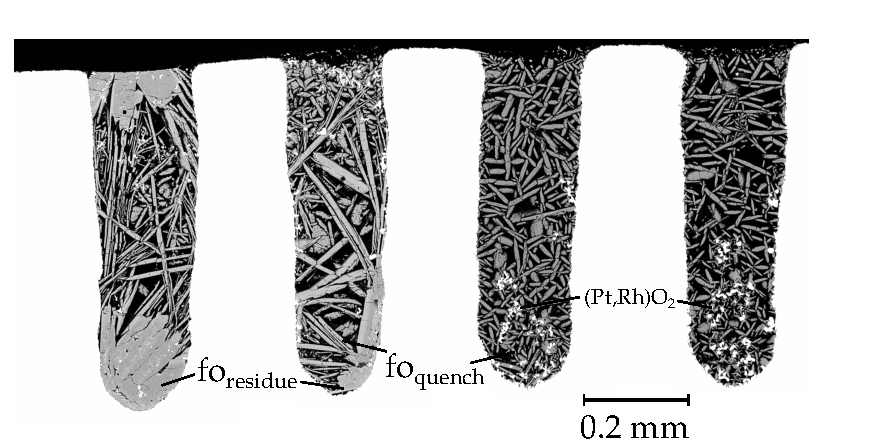
\includegraphics[width=0.8\textwidth]{figures/Z1058_1400C_13GPa_fo}
  \caption{BSE image of typical run products. Experimental chambers from Experiment Z1058, conducted at 1400 $^{\circ}$C and 13 GPa. Chambers have compositions along the forsterite-water binary, with water contents increasing from left to right.}
  \label{fig:sem}
\end{figure}


\section{Discussion}
\subsection{Modelling water solubility in melts}

Oxygen in MgO-SiO$_2$-H$_2$O melts can exist either as molecular water, as a bridging oxygen between magnesium and/or silicon atoms, or as part of a terminal hydroxyl group. The general equation describing the reaction between melt species is
\begin{equation}
0.5 \textrm{H}_2\textrm{O} + 0.5 \textrm{O}_{br}^{2-} \rightleftharpoons \textrm{OH}_{tm}^-
\label{eqn:speciation}
\end{equation}

where the subscripts br and tm respectively refer to bridging and terminal oxygens. The equilibrium between these species can be described with an equilibrium constant $K$ \cite[e.g.][]{Stolper1982}
\begin{equation}
K = \frac{X_{\textrm{OH}_{tm}^-}}{\sqrt{X_{\textrm{H}_2\textrm{O}} X_{\textrm{O}_{br}^{2-}} } }
\label{eqn:equilibrium_constant}
\end{equation}

The equilibrium constant is related to the energy $\Delta G^{\circ}$ required to protonate a bridging oxygen
\begin{equation}
K = \exp\left(\frac{-\Delta G^{\circ}}{RT}\right)
\end{equation}

These equations can be used to describe in an average sense a range of melt-melt equilibria involving monomers (Mg(OH)$_2$ and Si(OH)$_4$), dimers (Mg$_2$O(OH)$_2$, MgSiO(OH)$_4$, Si$_2$O(OH)$_6$) and higher oligomers. A high proportion of monomers and dimers exist in relatively dilute solutions, but not in the concentrated solutions investigated in this study.

A number of models have been presented to investigate the behaviour of concentrated hydrous melts. \cite{SS1985} made the assumption that H$_2$O, O$_{br}^{2-}$ and OH$_{tm}^-$ mix ideally, with a parameter $r$ representing the number of oxygen atoms in each formula unit which are available for protonation. For example, an Mg$_2$SiO$_4$ melt with $r=4$ and $K=\infty$ represents a continuum between an anhydrous melt and one made purely of monomers. If r is less then the number of oxygens per formula unit no distinction is made between isolated oligomers and partial depolymerisation of a silicate network; in other words, the energy required to form a terminal OH group is independent of local environment. Fixing $r$ places an implicit constraint on the maximum value of $K$ in water-rich compositions. For example, if $r=2$ in a hydrous forsteritic melt, then water contents exceeding 50\% require that $K<\infty$. In practise, the equilibrium constant $K$ has been shown to be dependent on temperature and composition. \cite{SK1995} obtained a good fit to isochemical data with an expression of the form
\begin{equation}
\Delta G^{\circ} = a + b\,T
\end{equation}

\cite{THH2012} simplified the model of \cite{SS1985} by assuming that all hydrogen in the melt exists as OH$^-$, and that protonation is equally likely on any oxygen ($K=\infty$, $\Delta G^{\circ}=-\infty$, $r$ maximised). Deviations from this model must increase with increasing water content, and such a model cannot describe any melt more water-rich than the Mg(OH)$_2$-Si(OH)$_4$ binary. 

To describe melting in the SiO$_2$-H$_2$O system, \cite{HM2012} generalised the  aforementioned models by allowing non-ideality between the two endmembers. The excess term $\Delta G^{\circ}$(P,T) for the formation of OH$^-$ groups was assumed to be independent of composition; all oxygens are equally available for protonation, and the local extent of protonation does not affect the energy required for each further protonation.

In all of these models, the activity of component $x$ with the composition of the liquidus phase $X$ can be calculated from the melt model and independently from the entropy of melting of $X$. At equilibrium, these two activities must be equal:
\begin{equation}
RT \ln a_{x,L}^X = G_{X_l} - G_{X_{s}} = - \int_T^{T_{melt}} S_{X_{l}}-S_{X_s} \, dT
\end{equation}
where $T_{melt}$ is the temperature of melting of the liquidus phase under anhydrous conditions.


\citep{NM2008}
\citep{DM2010}
\citep{ZK1998}

\subsection{Subsystems}
\subsubsection{MgO-H$_2$O}
The dehydration of brucite at high pressure was previously studied by \cite{FIYKFO2005}. They reported that the stability of brucite reaches a maximum at about 9--10 GPa and 1200 $^{\circ}$C, decomposing at 1100--1150 $^{\circ}$C at 13 GPa. We observed large brucite crystals at 1200 $^{\circ}$C and 13 GPa; so assuming that errors from both studies are $\sim$ 50 $^{\circ}$C, decomposition takes place just above 1200 $^{\circ}$C. In the present study, the composition of the fluid coexisting with brucite and periclase is constrained to be 64--66 mol\% H$_2$O. The MgO content of the fluid increases gradually with increasing pressure, as a result of the extremely high melting temperature of periclase. The best experimental estimate of the melting point of MgO is currently that of \cite{ZF2008}, who extrapolated to the MgO endmember using melting phase relations in the system (Mg,Fe)O. Their melting curve is essentially identical to that obtained from large-scale molecular dynamics simulations \citep{CG1994}. Using these two studes, melting at 13 GPa is estimated to be $\sim 5373$ K. This value is higher than that from more recent ab-initio investigations \citep{Alfe2005,KKS2013}, and 2000 K higher than the melting temperature estimated experimentally by \cite{ZB1994}.

At 13 GPa, the entropy of melting of periclase is estimated to be $\sim$22 J/K/mol \cite{CG1994}. Assuming that the metastable entropy of melting at this pressure remains constant with temperature, the activity of periclase in the system can be determined and used to fit a melting model to the experimental data. Using the ideal OH$^-$ mixing model of \cite{SS1985} with no compositional dependence on the formation of OH groups, $G^{\circ}= -70000 - 15T$ provides a good fit to the data. However, this model yields a low activity of water in equilibrium with brucite and periclase ($a_{H_2O}\sim 0.34$) relative to that estimated using the thermodynamic data of \citep{HP2011} and the equation of state of water formulated by \cite{PS1995} ($0.52$).

To simultaneously fit the melting data and the activity of water in melts in equilibrium with periclase and brucite, $\partial^2 G_{ex} / \partial X_{H_2O}^2$ needs to be less positive at compositions more water-rich than brucite. This can be achieved by imposing a binary subregular model (W$_{MgO-H_2O}$=38000 J/mol, W$_{H_2O-MgO}$=0 J/mol). This model also has the effect of increasing the tendency for melt-fluid immiscibility at the water-rich end of the system. The second critical endpoint of the MgO-H$_2$O is probably around 13 GPa \citep{MSUP2007}, so large positive interaction enthalpies are justified in this region of the phase diagram. Alternatively, a regular solution model with MgO, Mg(OH)$_2$ and H$_2$O species in the melt can adequately fit the data, with parameters G$_{br,melt} = -41000. - 10*(T-(1210.+273.15))$, W$_{MgO-H_2O}=0$, W$_{MgO-Mg(OH)_2}=-10000$, W$_{Mg(OH)_2-H_2O}=-22000$ (all in J/mol). The resulting fits are shown in Figure \ref{fig:MH}. The large differences between the two model-types at high temperature is a result of the much larger entropy of mixing in the \cite{SS1985} models close to the anhydrous endmembers.

\begin{figure}[ht!]
  \centering
      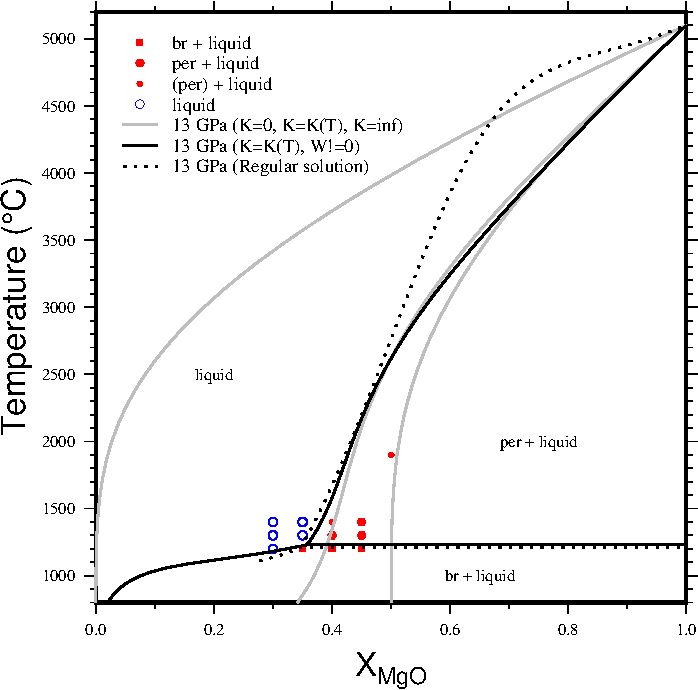
\includegraphics[width=0.8\textwidth]{figures/per-H2O}
  \caption{The periclase-water phase diagram at 13 GPa, based on current experimental results. The position of the dry periclase melting point is taken from \cite{ZF2008}, with an entropy of dry melting from \cite{CG1994}. Model fits in grey use the model of \cite{SS1985}, with r=1 and K=$\infty$ (bottom), K=K(T) (expression in main text) and K=0 (all H2O as molecular, top). The black line includes an interaction term to match the fluid in equilibrium with brucite during it's decomposition to periclase. The black dotted line represents a regular solution model with MgO, Mg(OH)$_2$ and H$_2$O as distinct species in the melt (parameters in the main text).}
  \label{fig:MH}
\end{figure}

\clearpage
\subsubsection{Mg$_2$SiO$_4$-H$_2$O}
The melting point depression of forsterite in the presence of water at 13 GPa is illustrated in Figure \ref{fig:foH}. The anhydrous melting of forsterite is incongruent. The temperature of the fo $\rightarrow$ per + L reaction is taken from \citep{PW1993}, with the temperature of the metastable fo $\rightarrow$ L reaction extrapolated from the same study. The liquidus is calculated by interpolation between the melting temperature of periclase \citep{ZF2008} and an estimate of the temperature and composition of melt in equilibrium with periclase and forsterite by interpolating between the invariant fo-per-foL point \citep{PW1993} and position of the per liquidus at 16 GPa \citep{LF2012}.

One chamber from an experiment run at 1300 $^{\circ}$C revealed a single very small crystal of enstatite. Another run at  $^{\circ}$C revealed large crystals of hydroxychondrodite in the chamber with the lowest water contents. Small differences in Mg:Si ratio could explain the differences in solid phases between the separate chambers, so it is assumed that the enstatite+forsterite and chondrodite+forsterite cotectics migrate very close to the forsterite+H$_2$O binary at high water contents and approximately 1200 $^{\circ}$C.

\begin{figure}[ht!]
  \centering
      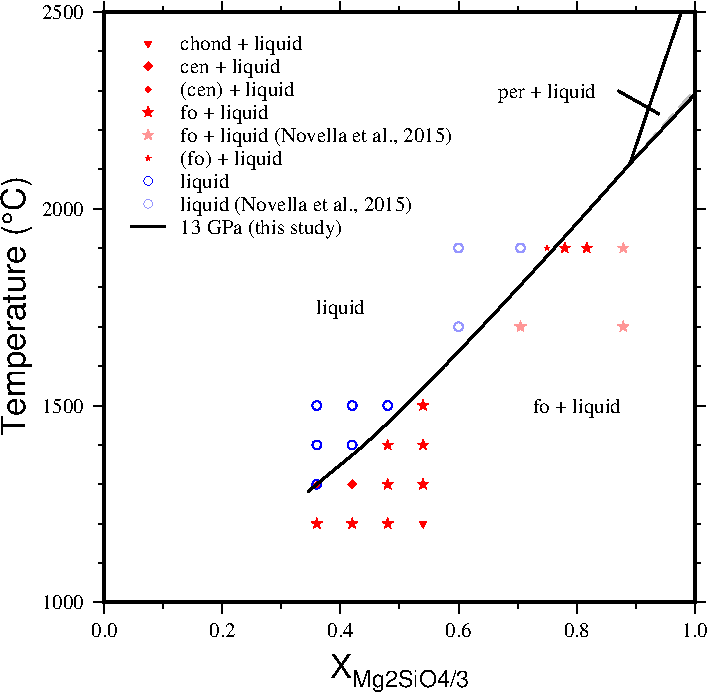
\includegraphics[width=0.8\textwidth]{figures/fo-H2O}
  \caption{The forsterite-water phase diagram at 13 GPa, based on current experimental results. The position of the dry melting point is taken from \citep{PW1993}. \citep{LF2012}.}
  \label{fig:foH}
\end{figure}
\clearpage
\subsubsection{MgSiO$_3$-H$_2$O}

The melting of clinoenstatite in the presence of water is shown in Figure \ref{fig:eoH}. The lack of stishovite as a liquidus phase is in agreement with \cite{YII2004}, who reported a clinoenstatite + stishovite + liquid field appearing at 13.5 GPa. 
\begin{figure}[ht!]
  \centering
      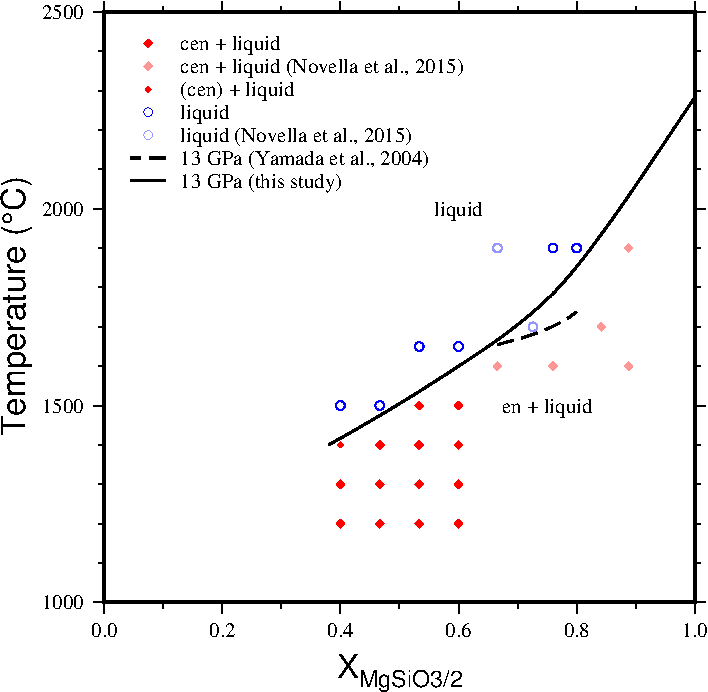
\includegraphics[width=0.8\textwidth]{figures/en-H2O}
  \caption{The clinoenstatite-water phase diagram at 13 GPa, based on current experimental results. The position of the dry melting point is taken from \cite{PG1990}.}
  \label{fig:eoH}
\end{figure}

\clearpage
\subsubsection{SiO$_2$-H$_2$O}
The 13 GPa SiO$_2$-H$_2$O binary phase diagram is shown in Figure \ref{fig:SH}. The anhydrous melting temperature of coesite and the temperature of the coesite-stishovite transition at 13 GPa are taken from \cite{ZLGHF1993}. The metastable melting temperature of stishovite is taken from the melting curve of \cite{Millotetal2015}, which is consistent with the shock data of \cite{LAM1983} and static melting data of \cite{ZLGHF1993}.

The liquidus in this system provides quite severe constraints on thermodynamics in the anhydrous system. Given that SiO$_2$-H$_2$O liquids approach ideality with increasing pressure and temperature \citep{HM2012}, we feel justified in using the ideal mixing model of \cite{SS1985}. Using this model constrains the entropy of melting of stishovite to be between about 8 and 19 J/K/mol, not significantly higher than room pressure values \citep{HM2012,ZLGHF1993}. A value of 13.5 J/K/mol with G$_{OH}$=35000-20T J/mol yields the model shown in Figure  \ref{fig:SH}. Unfortunately, these entropy values of are much higher than the values estimated from the melting curve of SiO$_2$. The melting curve of coesite has a negligable dT/dP at 13 GPa \citep{ZLGHF1993}, constraining the $\Delta$V of melting to be approximately zero. Using the volume of coesite at the coesite-stishovite-liquid triple junction as a proxy for the volume of the melt, published melting curves of stishovite \citep{Millotetal2015, ZLGHF1993} imply an entropy of melting of $\sim$120 J/K/mol. There are two potential resolutions to this problem. The first is that the assumptions of the hydrous melting model are inappropriate for the high pressure SiO$_2$ system. The second is that the thermodynamic properties in the anhydrous system need to be revisited. 

%NB: Most likely culprit the change in S with temperature?? Need a melt and solid model to test this.

% We use the formulation of \cite{HM2012} to model SiO$_2$-H$_2$O melts at 13 GPa. The volume of stishovite is taken from \cite{HP2011}. The melting curve of coesite at this pressure has $dT/dP \sim 0$ \citep{ZLGHF1993}, so the volume of anhydrous SiO$_2$ at this pressure is roughly equal to the volume of coesite via the Clausium-Clapeyron relation $dT/dP = \Delta V / \Delta S$. Using these volumes, the metastable entropy of melting of stishovite $\Delta S_{stv-L}$ is estimated as 8.5 J/K/mol. For completeness, we also calculate the melting point and entropy of melting of ice VII at 13 GPa from \emph{P-V-T} data collected along the melting curve \citep{FFH2004}.

\begin{figure}[ht!]
  \centering
      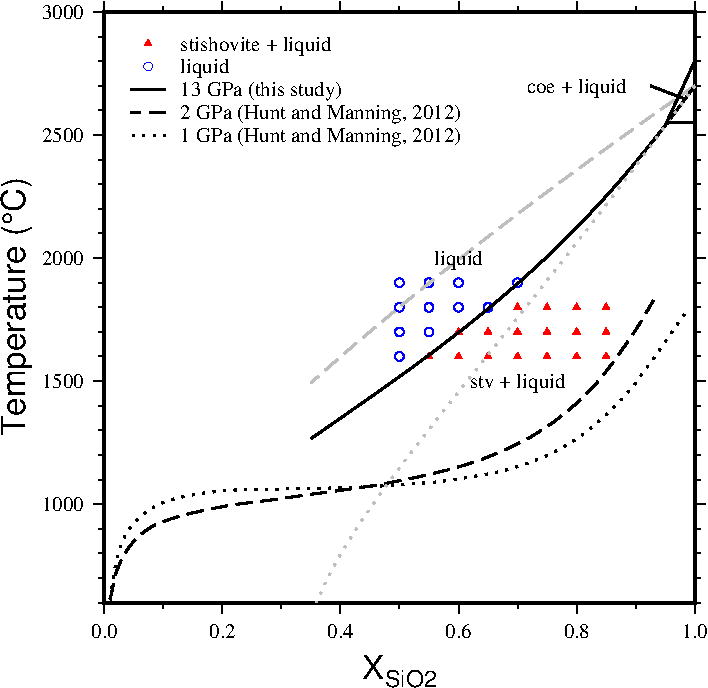
\includegraphics[width=0.8\textwidth]{figures/SiO2-H2O}
  \caption{The silica-water phase diagram at 13 GPa, based on current experimental results. The liquidus curve is compared with previous experimentally-derived models computed at 1 GPa and 2 GPa \citep{HM2012}. An entropy of 13.5 J/K/mol is chosen to fit the data. Model fits use the model of \cite{SS1985}, with r=2 and K=$\infty$ (dotted grey), K=K(T) (black, expression in main text) and K=0 (dashed grey, all H2O as molecular).}
  \label{fig:SH}
\end{figure}

%\citep{SU2001}
%\citep{KOM2005}
%\citep{AA1980}
%\citep{Inoue1994}
%\citep{Wunder1998}
%\citep{AFRH2001}
%\citep{Nagano2002}
%\citep{MSUP2007}
%\citep{MFY2002}
%\citep{Sta2004}
%\citep{MFY2004}
%\citep{SUTG2001}

\clearpage
\subsection{The MgO-SiO$_2$-H$_2$O system}
The set of experimental run products can be used to create a preliminary liquidus diagram (Figure \ref{fig:liquidus}).

\cite{YII2004} suggested that there was a sharp break in the liquidus at the enstatite-stishovite cotectic (their Figure 6). However, this prediction breaks Schreinemakers Rules (specifically, that no one assemblage can occupy more than 180$^{\circ}$ around an invariant point). 

\begin{figure}[ht!]
  \centering
      \includegraphics[width=0.8\textwidth]{figures/experimental-ternary}
  \caption{A preliminary liquidus diagram at 13 GPa, based on current experimental results.}
  \label{fig:liquidus}
\end{figure}

\subsection{Hydrous melting in high pressure subduction zone systems}
Subducting slabs are thought of transport significant quantities of mineral-bound water into the mantle transition zone. Much of this water is lost within the upper 200--300 km of the mantle through the breakdown of hydrous minerals such as antigorite and lawsonite. However, some mineral-bound water is thought to be preserved within a series of dense hydrous magnesium silicate (DHMS) phases. This observation was recently confirmed by the discovery of hydrous ringwoodite in diamond, which must have formed in the lower half of the mantle transition zone. The amount of water in the ringwoodite suggested that last equilibration occured under cold conditions probably associated with subduction. A key question, then, is how this material reached the surface sufficiently quickly to avoid retrogression to olivine, and how it remained cold during ascent to avoid the creation of hydrous melts. One effective way to allow melts to rapidly ascend to the surface is to channelise them. In turn, channelisation is promoted by reaction-infiltration and positive deformation-infiltration feedbacks. 

The results of this study provide important constraints on the relationships between hydrous melt and the surrounding environment under the conditions at the top of the mantle transition zone. Within a single lithology, melts percolating upwards into hotter surroundings will consume small amounts of the surrounding solids, encouraging channelisation. At such high pressures, the change in fluid composition with temperature is gradual along the forsterite-enstatite and enstatite-stishovite cotectics, and the stishovite melting curve. Thus, it is unlikely that melt fraction will rapidly change in a single lithology.

A more profound effect occurs when hydrous fluids in equilibrium with peridotites infiltrate more Si-rich rocks. The enstatite-stishovite cotectic has a much greater $\partial T/\partial X_{H_2O}$ than the forsterite-enstatite cotectic at high temperatures. This implies that fluids entering silica-rich rocks will be corrosive, consuming enstatite and stishovite to reach equilibrium with their new surroundings. Despite being volumetrically minor components of subduction zone systems, silica-rich lithologies could play a dominant role in channelising hydrous fluids. The motion of these fluids could also significantly weaken the uppermost slab, effectively decoupling it from the overlying mantle wedge. Such effects promote trench parallel flow, encouraging slab deformation and rollback (trench migration relative to the surrounding mantle).



\clearpage
\section*{References}

\bibliography{references_MSH}

\end{document}
